\documentclass[12pt,a4paper, twosite]{article}
\usepackage{mystyle}

%oben und unten
\usepackage{fancyhdr}
\pagestyle{fancy}
\lhead{St. Michael\\Fribourg}
\rhead{Labor: Optische Geräte}
\rfoot{Felix Binder}
\lfoot{Dezember 2013}
\renewcommand\headrulewidth{1pt}
\renewcommand\footrulewidth{1pt}
%ende oben und unten


\author{}
\date{}
\title{Optische Geräte}

\begin{document}
\maketitle
%\thispagestyle{empty}

\section*{Material}
Für diesen Praktikumstag werden folgende Materialien benötigt:
\begin{itemize}
	\item Optische Bank mit Linsen 
	\item Experimentiertischchen
	\item Lineal
\end{itemize}

\section*{Vorbereitung und Versuchsaufbau}

\begin{itemize}
%	\item Entfernen Sie alle Komponenten von der optischen Bank.
	\item Montiere Sie die Linse mit der Brennweite von $f=\SI{5}{cm}$ und einen Schirm auf der optischen Bank.
\end{itemize}


%\begin{figure}[t]
%	\begin{center}
%	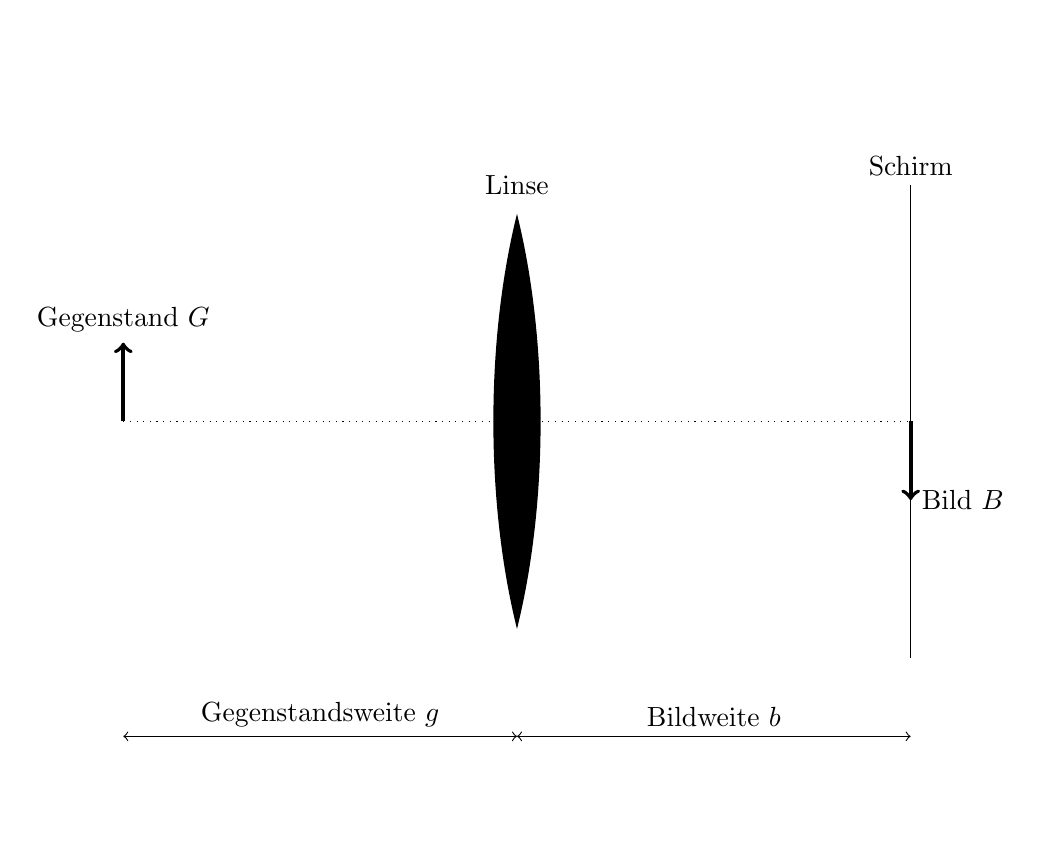
\begin{tikzpicture}

%Mittellinie
\draw [dotted] (-5,0)--(5,0);

%Gegenstand
\draw [->=latex, line width=0.05cm] (-5,0)--(-5,1) node [above] {Gegenstand $G$};
%Bild
\draw [->=latex, line width=0.05cm] (5,0)--(5,-1) node [right] {Bild $B$};

\begin{scope}[xscale=2, yscale=5]
\clip (-0.85,0) circle (1cm);
\clip (0.85,0) circle (1cm);
\fill(-2,-2) rectangle (2,2);
\end{scope}

\draw (0,3) node {Linse};

%Schirm
\draw (5,-3)--(5,3) node [above] {Schirm};


\draw [<->=latex] (-5,-4)--(0,-4) node [midway, above] {Gegenstandsweite $g$};
\draw [<->=latex] (0,-4)--(5,-4) node [midway, above] {Bildweite $b$};
\end{tikzpicture}
%	\caption{\label{fig1} Skizze des Versuchsaufbaus.} 
%	\end{center}
%\end{figure}



\section*{Versuch: Auge mit Brille}
\begin{itemize}
	\item Bauen Sie ein Modell eines weitsichtigen Auges. Dazu verändern Sie den Abstand 
		Linse -- Schirm so, dass weit entfernte Objekte auf dem Schirm scharf abgebildet werden.
	\item Versuchen Sie die Fehlsichtigkeit des Augenmodells durch eine ``Brille'' zu korrigieren.
		Welche Form hat die Korrekturlinse? Konvex oder konkav?
	\item Wiederholen Sie das Experiment für ein kurzsichtiges Auge.
\end{itemize}


\section*{Versuch: Sehwinkel und Teleskop}
\begin{itemize}
	\item Schauen Sie aus dem Fenster und suchen Sie sich ein Objekt in der Ferne.
	\item Bestimmen Sie den Sehwinkel $\epsilon$, unter dem Sie das Objekt sehen.
	\item Bauen Sie ein Teleskops. Stecken Sie dazu die Linse mit \SI{30}{cm} Brennweite (Objektiv) und einen Schirm auf die optische Bank.
	\item Versuchen Sie das Bild ihres Objekts auf dem Schirm abzubilden. Wie gross ist die Bildweite?
	\item Entfernen Sie den Schirm und betrachten Sie das ``Bild'' durch eine zweite Linse (Okular) mit kleinerer Brennweite.
	\item Versuchen Sie den Sehwinkel durch das Teleskop zu bestimmen.
	\item Was ändert sich wenn Sie eine konkave Linse als Okular benutzen?
\end{itemize}

\section*{Zusammenfassung}
\begin{itemize}
	\item Was haben Sie im Praktikum gemacht?
	\item Wie korrigiert man Kurzsichtigkeit / Weitsichtigkeit?
	\item Was haben Sie beim Teleskop gelernt?
\end{itemize}

\end{document}
